\documentclass[aspectratio=169,hyperref={pdfusetitle,pdfencoding=auto}]{beamer}

% Language setup (if needed, via custom config)
\newif\ifgerman
\germantrue

\ifgerman
  \def\babellanguage{ngerman}
  \def\polyglossialanguage{german}
  \def\biblatexsorting{de_DE}
\else
  \def\babellanguage{english}
  \def\polyglossialanguage{english}
  \def\biblatexsorting{en_US}
\fi

\usepackage{../cd-theme/cd-fub-theme}

\titlegraphic{\FUlogo[1cm]{../logos/fu-rgb-green-boxes.png}}
\title[Demo]{FU Berlin Corporate Design – Demo}
\author[Initials]{Your Name}
\date{\today}

\AtBeginSection[]
{
\begin{frame}
  \frametitle{Table of Contents}
  \tableofcontents[currentsection]
\end{frame}
}

\pgfdeclareimage[width=3cm]{logo}{./Fub-logo_svg.png}
\logo{\pgfuseimage{logo}}

\title{An example title}
\subtitle{With a longer subtitle}
\institute{Institute for Silly Walks}
\author{Leonard König\and Foo Bar}

\begin{document}

% Example content

\begin{frame}
  \titlepage
\end{frame}

\begin{frame}{Overview}
  \tableofcontents
\end{frame}


\section{Introduction}

\begin{frame}{Overview of topic}
This should give a neat introduction about what were speaking about.
\begin{itemize}
  \item Foo
  \item Bar \enquote{baz} buzz
  \item Buzz buss
  \item La li lo
\end{itemize}

\begin{figure}
\centering
\resizebox{!}{.3\textheight}{
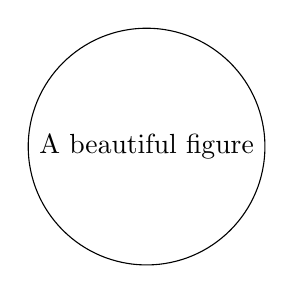
\begin{tikzpicture}[every node/.style={draw,circle}]
  \node {A beautiful figure};
\end{tikzpicture}
}
\caption{Caption of figure}
\end{figure}
\end{frame}


\subsection{Current Research}

\begin{frame}{An Example Research Method}
We now give overviews about current research methods.

\vfill
Note:
\begin{enumerate}
  \item If we need to cite, we can do this~\cite{Author/2025}
  \item We can keep \enquote{hide} these\nocite{Author/2025}
  \item They still show up in the bibliography
\end{enumerate}
\vfill
\end{frame}

